\section{Análisis del problema}

El principal problema que nos concierne es la detección y separación del grano contaminado de la corriente de cereal circulando por los transportadores. Para solucionarlo,
la propuesta de sistema a implementar consiste en la instalación de cámaras infrarojas en la línea de procesado, capaces de captar las imágenes hiperespectrales de la
corriente. De manera que utilizando nuestro modelo previamente calibrado, se detecte cuáles son los granos más contaminados y se puedan separar mediante una corriente de aire. 
Podemos ver un esquema del prototipo del sistema en la \textit{Figura\ \ref{fig:detection-system}}.

\begin{figure}[!h]
    \centering
    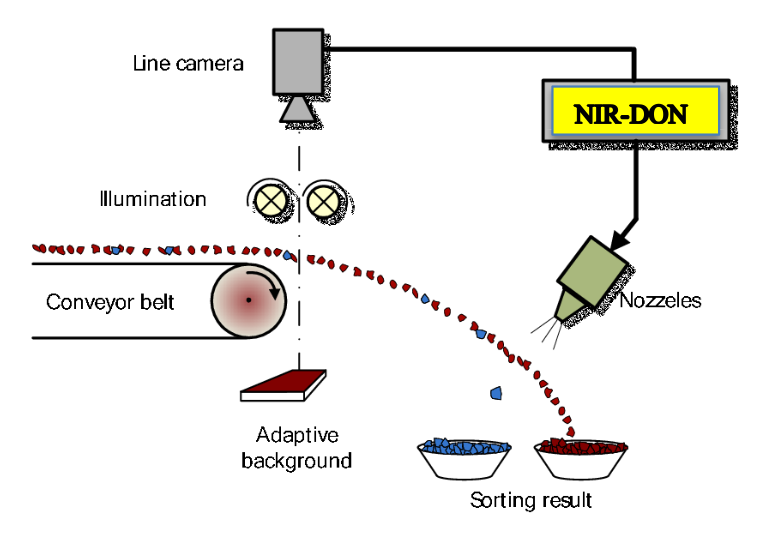
\includegraphics[width=0.7\linewidth]{media/images/esquema-del-sistema.png}
    \caption{Esquema del sistema de detección y filtrado de granos contaminados}\ \label{fig:detection-system}
\end{figure}


\subsection{NIR-HSI}


\gls{nir-hsi} es una tecnología rápida, no destructiva y precisa que nos permite hacer inspecciones de calidad, la cual ha demostrado su potencial en los últimos años\ \cite{Applicat5:online}. 
Es una técnica de imagen química basada en la espectroscopia de reflectancia (la luz reflejada por los materiales), la cual es capaz de caracterizar compuestos orgánicos y algunos minerales\ \cite{NIRHyper23:online}. Comparado con el análisis químico por lotes, el método propuesto puede resultar mucho más directo, pues es rápido, barato, y preciso; pues permite analizar los granos individualmente y en tiempo real y no en lotes analizados en diferido.

Como hemos comentado en la introducción, nuestro objetivo es conseguir un modelo que, utilizando \gls{nir-hsi}, prediga lo mejor posible qué granos de una \gls{imagen hiperespectral} están contaminados con \acrshort{don}. Para ello, partimos con una base de datos de imágenes hiperespectrales en formato \acrshort{bil}, las cuales simulan las imágenes tomadas en la cadena de producción y de las cuáles podemos extraer la información de los píxeles que forman los granos.
Los archivos con formato \acrshort{bil} albergan los datos hiperespectrales de una imagen, tal como se muestra en la \textit{Figura \ref{fig:bil-example}}. Para ello, se hace uso de otro archivo complementario con formato \textit{bil.hdr} el cual brinda información extra, como, por ejemplo, las diferentes bandas (frecuencias de onda) presentes en la imagen. 

\begin{figure}[!ht]
    \centering
    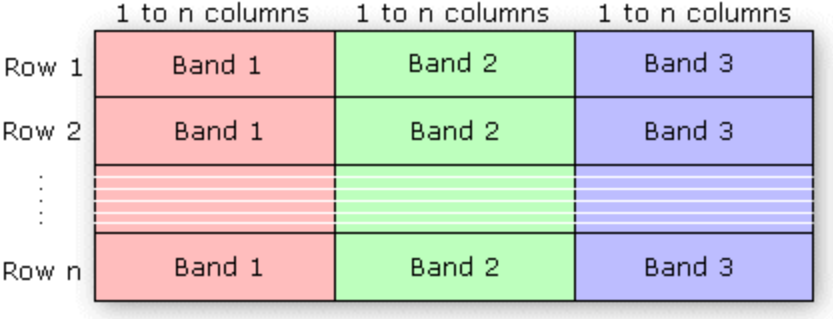
\includegraphics[width=0.7\linewidth]{media/images/bil.png}
    \caption{Formato de los datos en un archivo \acrshort{bil}. Fuente \cite{Archivos82:online}}\ \label{fig:bil-example}
\end{figure}

Una vez sabemos qué formato tienen los datos, podemos leer los archivos \acrshort{bil} que tenemos y formar un \acrshort{csv} con los datos centralizados para que nos sea más cómodo trabajar con ellos. Para no tener un archivo demasiado grande, hemos desechado los píxeles que forman parte del `fondo' negro de la imagen, para determinar si un píxel es parte del grano o del fondo, se calcula la media de los valores de las reflectancias para ese píxel y si no pasa un umbral de , lo consideramos parte del fondo.

Una vez tenemos el \acrshort{csv} con los datos de cada píxel, podemos generar un nuevo \gls{dataset} que agrupe los píxeles en grupos, o granos. De esta forma, podemos añadir un nuevo filtro que consista en que los granos deben de tener un tamaño mínimo (número de píxeles), es decir, podemos desechar los granos que sean demasiado pequeños ya que probablemente sea ruido en la imagen. De esta forma, agruparíamos \textit{N} filas de datos de píxeles, en tan solo una fila conservando la media de cada columna.

Por otro lado, tenemos una base de datos con el estado de contaminación de estos mismos granos. A partir de ahora utilizaremos los términos contaminación y etiqueta como sinónimos a la hora de referirnos a los granos.


\subsection{Contaminación del grano}\ \label{sec:separacion}

El valor de contaminación \acrshort{don} de una muestra se obtiene, como hemos comentado anteriormente, realizando un análisis químico por lotes. Este análisis nos devuelve el valor de la concentración de \acrshort{don} en el lote, de modo que si supera los \(1250\ \mu g/kg\), por ley, la muestra se considera contaminada. Sabiendo esto, previamente en laboratorio se ha realizado un análisis de los granos que forman las imágenes \acrshort{bil} que tenemos y, por lo tanto, además de los datos hiperespectrales, sabemos el nivel de contaminación que posee cada grano y lo podemos agregar como columna en el \acrshort{csv} que tenemos.


Al ser el valor de contaminación el que queremos predecir, a partir de ahora utilizaremos los términos contaminación y etiqueta como sinónimos. Además agregaremos otra columna, también de contaminación, la cual será \textit{booleana}, en lugar de un valor contínuo, y nos indicará si el valor concentración de ese grano supera el umbral legal comentado anteriormente. De esta forma, podríamos plantear el problema tanto por regresión como por clasificación, sin embargo, lo enfocaremos en la clasificación, pues no nos interesa saber el grado de contaminación de un grano, sino si está contaminado o no. 
